%!TEX root=../protocol.tex	% Optional

\section{Zadání}
Na předloženém přípravku vyzkoušejte následující funkce číslicového osciloskopu:

\subsection{Základní nastavení osciloskopu}
Zobrazte signál č. 1 přípravku na osciloskopu pomocí funkce \textit{Autoset}. Nastavte zobrazení tak, aby zobrazeny byly cca 2 periody signálu a rozkmit signálu byl téměř přes celou výšku displeje.

\subsection{Měření a Zoom}
Změřte základní parametry signálu - $V_{pp}$, periodu, frekvenci, $U_{Avg}$, $U_{RMS}$. Zjistěte vliv AC/DC vazby vstupu na měřené hodnoty. V režimu \textbf{\textit{Single}} změřte rychlost náběžné a spádové hrany pulsu.

\subsection{Využití funkce hold-off}
Zasynchronizujte zobrazení signálu č. 3 přípravku s využitím interního spouštění a funkce hold-off osciloskopu. Zdůvodněte, proč právě Vámi zvolená délka časového intervalu hold-off je ta správná.

\subsection{Spouštění šírkou pulsu}
Zasynchronizujte signál č. 3 s využitím spouštění od minimální šířky pulsu ( > ). Pozorujte glitch, ve čtvrtém pulsu úrovně log. 1 v sekvenci, pro detailní pozorování zvolte možnost spouštění od maximální šířky pulsu ( < ). V obou případech uveďte nastavenou spouštěcí podmínku a zdůvodněte, proč díky ní osciloskop správně synchronizuje.

\subsection{Měření šírky pulsu}
Pomocí funkce automatického měření změřte šířku glitch pulsu v signálu č. 3.

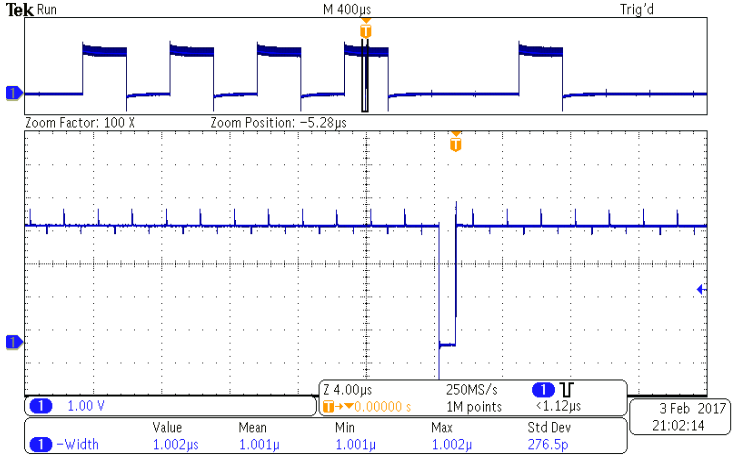
\includegraphics[width=0.87\textwidth]{images/05-zadani.png}

\subsection{Měření zpoždění}
Na vstupy osciloskopu přiveďte signály č. 5 a č. 6, osciloskop zasynchronizujte (můžete využít tlačítko AUTOSET). Pomocí funkce automatického měření změřte zpoždění (delay) mezi náběžnými a poté mezi sestupnými hranami těchto signálů.

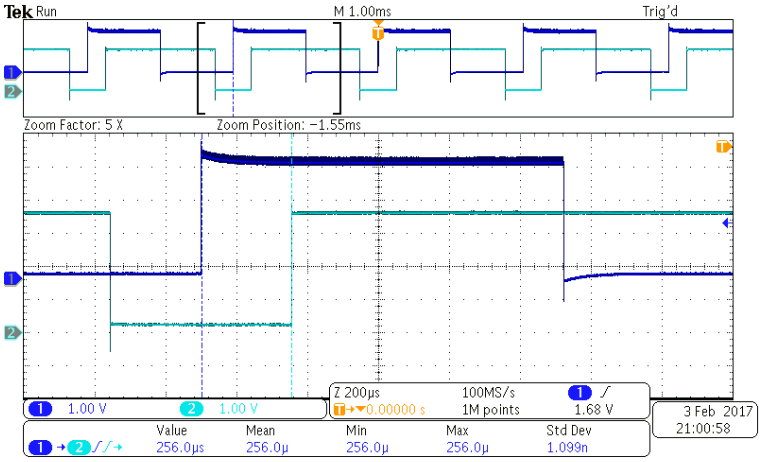
\includegraphics[width=0.87\textwidth]{images/06-zadani.png}

\subsection{Spouštění runt pulsem}
Signál č. 8 obsahuje puls s nižší napěťovou úrovní pro log.1 (pravděpodobná kolize dvou budičů, kdy jeden generuje úroveň log.1 a druhý log.0). Nastavte osciloskop tak, aby spouštěl od výskytu tohoto pulsu (runt) a poté změřte pomocí funkce automatického měření napěťovou úroveň odpovídající log. 1 u běžného i kolizního pulsu.

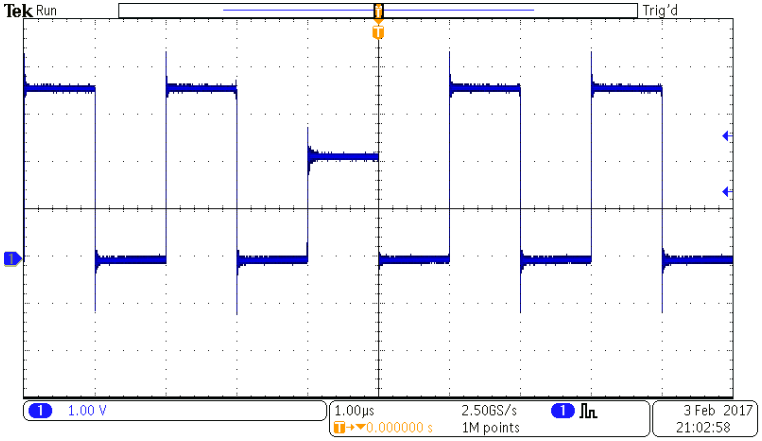
\includegraphics[width=0.87\textwidth]{images/07-zadani.png}

\subsection{Spouštění délkou hrany pulsu}
Signál č. 9 obsahuje puls s delšími hranami, než mají ostatní pulsy (degradace či nevhodná technologie jednoho z budičů na sběrnici). Nastavte osciloskop tak, aby spouštěl od výskytu tohoto pulsu a poté změřte pomocífunkce automatického měření rychlost náběžné a sestupné hrany standardního i degradovaného pulsu.

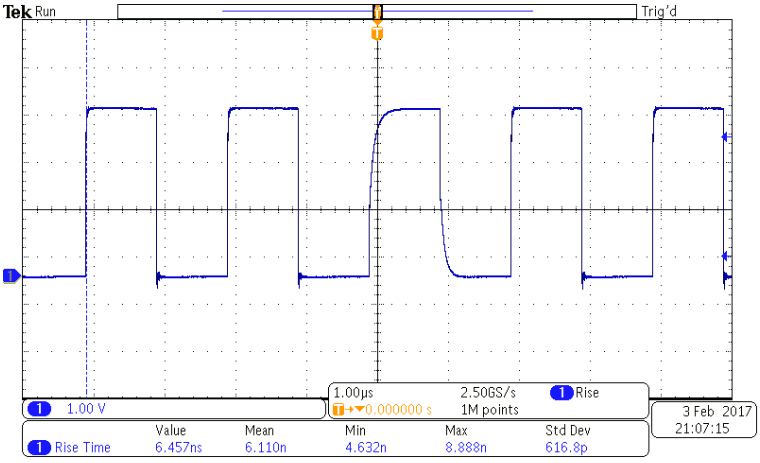
\includegraphics[width=0.87\textwidth]{images/08-zadani.png}